% Options for packages loaded elsewhere
\PassOptionsToPackage{unicode}{hyperref}
\PassOptionsToPackage{hyphens}{url}
%
\documentclass[
]{article}
\usepackage{amsmath,amssymb}
\usepackage{lmodern}
\usepackage{iftex}
\ifPDFTeX
  \usepackage[T1]{fontenc}
  \usepackage[utf8]{inputenc}
  \usepackage{textcomp} % provide euro and other symbols
\else % if luatex or xetex
  \usepackage{unicode-math}
  \defaultfontfeatures{Scale=MatchLowercase}
  \defaultfontfeatures[\rmfamily]{Ligatures=TeX,Scale=1}
\fi
% Use upquote if available, for straight quotes in verbatim environments
\IfFileExists{upquote.sty}{\usepackage{upquote}}{}
\IfFileExists{microtype.sty}{% use microtype if available
  \usepackage[]{microtype}
  \UseMicrotypeSet[protrusion]{basicmath} % disable protrusion for tt fonts
}{}
\makeatletter
\@ifundefined{KOMAClassName}{% if non-KOMA class
  \IfFileExists{parskip.sty}{%
    \usepackage{parskip}
  }{% else
    \setlength{\parindent}{0pt}
    \setlength{\parskip}{6pt plus 2pt minus 1pt}}
}{% if KOMA class
  \KOMAoptions{parskip=half}}
\makeatother
\usepackage{xcolor}
\IfFileExists{xurl.sty}{\usepackage{xurl}}{} % add URL line breaks if available
\IfFileExists{bookmark.sty}{\usepackage{bookmark}}{\usepackage{hyperref}}
\hypersetup{
  pdftitle={Comparison of intrinsic excitability of mPFC PN between CHD8 genotypes:::Action Potential Analysis},
  pdfauthor={KimYG},
  hidelinks,
  pdfcreator={LaTeX via pandoc}}
\urlstyle{same} % disable monospaced font for URLs
\usepackage[margin=1in]{geometry}
\usepackage{graphicx}
\makeatletter
\def\maxwidth{\ifdim\Gin@nat@width>\linewidth\linewidth\else\Gin@nat@width\fi}
\def\maxheight{\ifdim\Gin@nat@height>\textheight\textheight\else\Gin@nat@height\fi}
\makeatother
% Scale images if necessary, so that they will not overflow the page
% margins by default, and it is still possible to overwrite the defaults
% using explicit options in \includegraphics[width, height, ...]{}
\setkeys{Gin}{width=\maxwidth,height=\maxheight,keepaspectratio}
% Set default figure placement to htbp
\makeatletter
\def\fps@figure{htbp}
\makeatother
\setlength{\emergencystretch}{3em} % prevent overfull lines
\providecommand{\tightlist}{%
  \setlength{\itemsep}{0pt}\setlength{\parskip}{0pt}}
\setcounter{secnumdepth}{-\maxdimen} % remove section numbering
\ifLuaTeX
  \usepackage{selnolig}  % disable illegal ligatures
\fi

\title{Comparison of intrinsic excitability of mPFC PN between CHD8
genotypes:::Action Potential Analysis}
\author{KimYG}
\date{2022 June 17th}

\begin{document}
\maketitle

\hypertarget{analysis-for-ap-paramenters}{%
\subsection{Analysis for AP
paramenters}\label{analysis-for-ap-paramenters}}

\hypertarget{load-packages}{%
\subsubsection{0. Load packages}\label{load-packages}}

\hypertarget{load-depolarizing-current-injection-data-from-google-drive}{%
\subsubsection{1. Load depolarizing-current injection data from Google
drive}\label{load-depolarizing-current-injection-data-from-google-drive}}

\begin{verbatim}
## 'data.frame':    64 obs. of  14 variables:
##  $ CellID             : Factor w/ 64 levels "220503_WT_F_#03_L5",..: 1 2 3 4 5 6 7 8 9 10 ...
##  $ AP.threshold       : num  -39 -39.5 -35.9 -38.3 -40.8 ...
##  $ VelocityATthrehold : num  5.19 6.1 6.1 6.41 5.49 ...
##  $ Upstroke.V         : num  201 278 146 255 223 ...
##  $ Dowstroke.V        : num  -39.1 -52.8 -38.8 -47.6 -51 ...
##  $ AP.Amplitude       : num  76.4 83.3 64.2 82.3 80.5 ...
##  $ AHP.Amplitude      : num  2.9 6.23 4.21 3.94 7.69 ...
##  $ FWHM               : num  1.67 1.36 1.67 1.44 1.39 ...
##  $ Rin                : num  112.4 110.3 117.6 97.6 97.9 ...
##  $ Rheobase.current   : num  100 50 100 50 150 100 100 50 100 150 ...
##  $ Max_firing_step    : num  500 400 500 500 400 450 600 500 500 400 ...
##  $ FI_curve_slope     : num  0.0415 0.0481 0.044 0.0292 0.0674 ...
##  $ LastFirst_ISI_ratio: num  3.96 3.07 3.77 4.49 4.19 ...
##  $ group              : Factor w/ 4 levels "WT_F_L5","WT_M_L5",..: 1 1 1 1 1 1 1 1 1 1 ...
\end{verbatim}

\hypertarget{discriptive-statistics}{%
\subsubsection{2. Discriptive statistics}\label{discriptive-statistics}}

\begin{verbatim}
##                         Group  N         mean           SD          SEM
## AP.threshold.1        WT_F_L5 16 -31.11648550  10.28049526  2.570123815
## AP.threshold.2        WT_M_L5 17 -30.48167512   7.58536212  1.839720543
## AP.threshold.3        KO_F_L5 17 -36.10947553   6.72933818  1.632104242
## AP.threshold.4        KO_M_L5 14 -29.31649350   6.35786887  1.699211930
## VelocityATthrehold.1  WT_F_L5 16   6.50405888   2.05692025  0.514230061
## VelocityATthrehold.2  WT_M_L5 17   6.26507929   1.21169408  0.293878982
## VelocityATthrehold.3  KO_F_L5 17   6.92928535   1.64258832  0.398386184
## VelocityATthrehold.4  KO_M_L5 14   6.14711214   0.62033071  0.165790356
## Upstroke.V.1          WT_F_L5 16 241.79458619  64.11129626 16.027824065
## Upstroke.V.2          WT_M_L5 17 245.81011594  47.61831666 11.549138195
## Upstroke.V.3          KO_F_L5 17 248.59260118  66.41150722 16.107156414
## Upstroke.V.4          KO_M_L5 14 260.03156371  31.35642494  8.380357072
## Dowstroke.V.1         WT_F_L5 16 -53.31039419  11.42989223  2.857473057
## Dowstroke.V.2         WT_M_L5 17 -62.79440488  12.38621307  3.004097928
## Dowstroke.V.3         KO_F_L5 17 -63.85354435  13.44052891  3.259807079
## Dowstroke.V.4         KO_M_L5 14 -59.00791714   7.27574588  1.944524880
## AP.Amplitude.1        WT_F_L5 16  78.27949519   6.21188255  1.552970637
## AP.Amplitude.2        WT_M_L5 17  78.56122182   6.18915349  1.501090211
## AP.Amplitude.3        KO_F_L5 17  79.94169335   6.77437075  1.643026244
## AP.Amplitude.4        KO_M_L5 14  81.22253421   3.91183507  1.045481899
## AHP.Amplitude.1       WT_F_L5 16   3.56292725   2.77092218  0.692730546
## AHP.Amplitude.2       WT_M_L5 17   7.77480165   3.67965514  0.892447458
## AHP.Amplitude.3       KO_F_L5 17   4.80562106   4.30145136  1.043255194
## AHP.Amplitude.4       KO_M_L5 14   5.00488279   3.59436377  0.960634125
## FWHM.1                WT_F_L5 16   1.36793056   0.24183730  0.060459326
## FWHM.2                WT_M_L5 17   1.23859229   0.21064953  0.051090015
## FWHM.3                KO_F_L5 17   1.25316329   0.23091016  0.056003939
## FWHM.4                KO_M_L5 14   1.25779821   0.11359875  0.030360543
## Rin.1                 WT_F_L5 16  97.81505506  25.31306109  6.328265272
## Rin.2                 WT_M_L5 17 106.97603571  44.53082951 10.800312570
## Rin.3                 KO_F_L5 17 100.70735424  39.84207154  9.663121724
## Rin.4                 KO_M_L5 14  90.34971136  24.36903379  6.512898235
## Rheobase.current.1    WT_F_L5 16 146.87500000  88.44725358 22.111813396
## Rheobase.current.2    WT_M_L5 17 152.94117647  83.79772565 20.323933766
## Rheobase.current.3    KO_F_L5 17 161.76470588  96.06217349 23.298499291
## Rheobase.current.4    KO_M_L5 14 142.85714286  58.36602956 15.598977546
## Max_firing_step.1     WT_F_L5 16 493.75000000  68.00735254 17.001838136
## Max_firing_step.2     WT_M_L5 17 467.64705882 142.45742398 34.551000366
## Max_firing_step.3     KO_F_L5 17 444.11764706 134.49251018 32.619225019
## Max_firing_step.4     KO_M_L5 14 503.57142857 110.00749225 29.400738999
## FI_curve_slope.1      WT_F_L5 16   0.05732763   0.03182416  0.007956041
## FI_curve_slope.2      WT_M_L5 17   0.05108724   0.04283115  0.010388079
## FI_curve_slope.3      KO_F_L5 17   0.05921300   0.03698421  0.008969990
## FI_curve_slope.4      KO_M_L5 14   0.06050493   0.03636307  0.009718439
## LastFirst_ISI_ratio.1 WT_F_L5 16   4.63447819   0.75170489  0.187926223
## LastFirst_ISI_ratio.2 WT_M_L5 17   4.54331771   1.37386992  0.333212400
## LastFirst_ISI_ratio.3 KO_F_L5 17   5.55986641   2.00020954  0.485122070
## LastFirst_ISI_ratio.4 KO_M_L5 14   4.65262771   1.18994022  0.318024901
##                                CI
## AP.threshold.1         5.47808924
## AP.threshold.2         3.90003333
## AP.threshold.3         3.45990643
## AP.threshold.4         3.67092419
## VelocityATthrehold.1   1.09605543
## VelocityATthrehold.2   0.62299561
## VelocityATthrehold.3   0.84454098
## VelocityATthrehold.4   0.35816829
## Upstroke.V.1          34.16249832
## Upstroke.V.2          24.48307926
## Upstroke.V.3          34.14564624
## Upstroke.V.4          18.10466075
## Dowstroke.V.1          6.09055965
## Dowstroke.V.2          6.36840312
## Dowstroke.V.3          6.91048230
## Dowstroke.V.4          4.20089060
## AP.Amplitude.1         3.31007856
## AP.Amplitude.2         3.18216909
## AP.Amplitude.3         3.48306004
## AP.Amplitude.4         2.25862633
## AHP.Amplitude.1        1.47652021
## AHP.Amplitude.2        1.89190410
## AHP.Amplitude.3        2.21160222
## AHP.Amplitude.4        2.07532385
## FWHM.1                 0.12886600
## FWHM.2                 0.10830599
## FWHM.3                 0.11872305
## FWHM.4                 0.06558997
## Rin.1                 13.48837814
## Rin.2                 22.89563985
## Rin.3                 20.48490295
## Rin.4                 14.07026121
## Rheobase.current.1    47.13021461
## Rheobase.current.2    43.08481489
## Rheobase.current.3    49.39061211
## Rheobase.current.4    33.69954216
## Max_firing_step.1     36.23856017
## Max_firing_step.2     73.24484877
## Max_firing_step.3     69.14966797
## Max_firing_step.4     63.51643501
## FI_curve_slope.1       0.01695790
## FI_curve_slope.2       0.02202174
## FI_curve_slope.3       0.01901553
## FI_curve_slope.4       0.02099541
## LastFirst_ISI_ratio.1  0.40055526
## LastFirst_ISI_ratio.2  0.70637873
## LastFirst_ISI_ratio.3  1.02841285
## LastFirst_ISI_ratio.4  0.68705103
\end{verbatim}

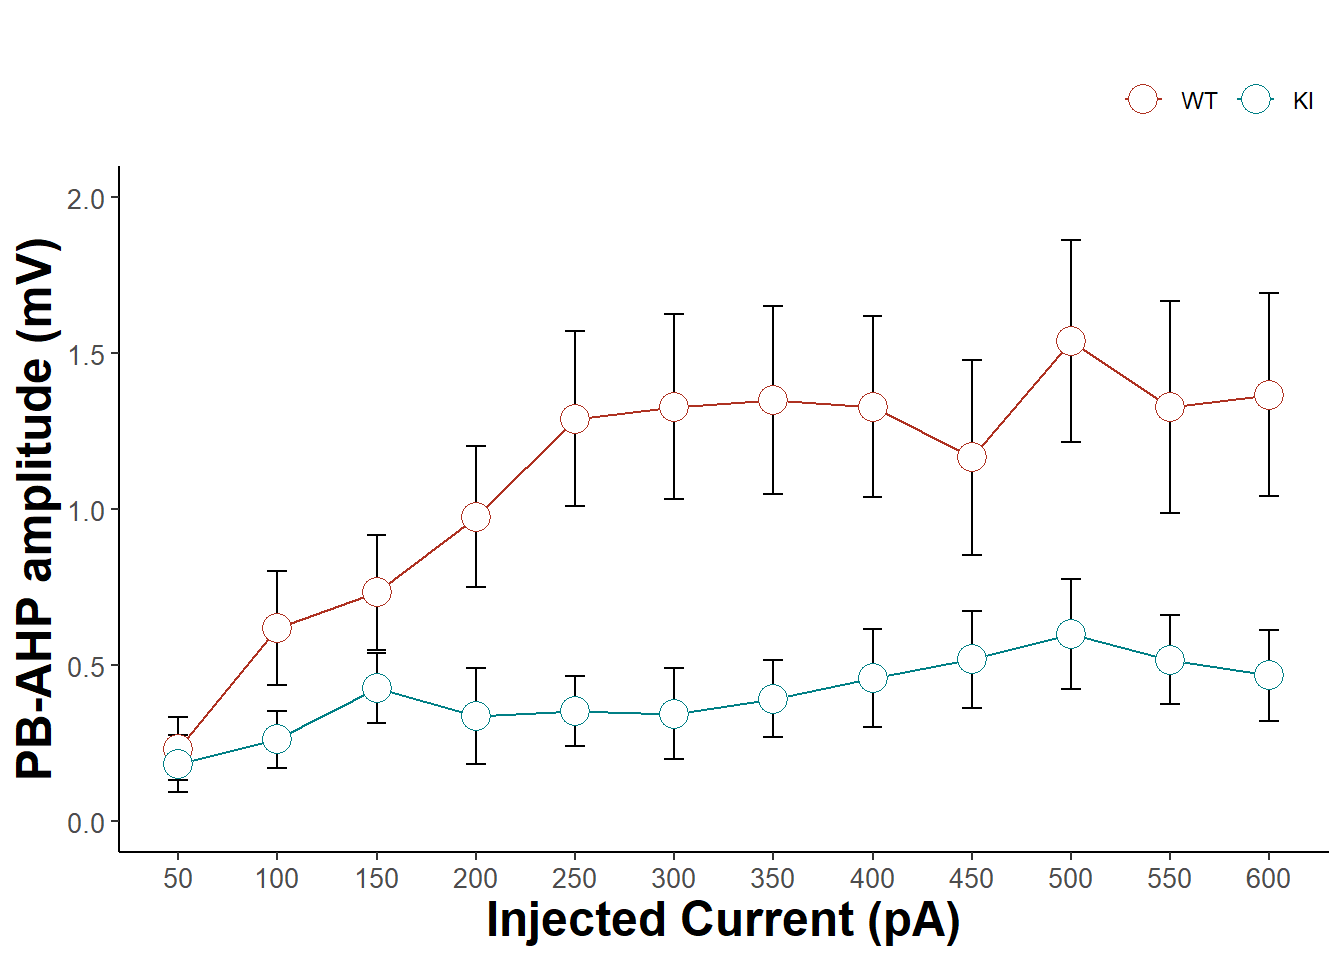
\includegraphics{220616_AP-Analysis_L5_Four-groups_files/figure-latex/unnamed-chunk-6-1.pdf}

\end{document}
